
\item \points{25} {\bf Reinforcement Learning: The inverted pendulum}
\\\\
{\bf Problem Setup}

In this problem, you will apply reinforcement learning to automatically
design a policy for a difficult control task, without ever using any 
explicit knowledge of the dynamics of the underlying system.

The problem we will consider is the inverted pendulum or the pole-balancing 
problem.\footnote{The dynamics are adapted from {\tt
    http://www-anw.cs.umass.edu/rlr/domains.html}}

Consider the figure shown. A thin pole is connected via a free hinge to a cart, 
which can move laterally on a smooth table surface. The controller is said to 
have failed if either the angle of the pole deviates by more than a certain
amount from the vertical position (i.e., if the pole falls over), or if the
cart's position goes out of bounds (i.e., if it falls off the end of the table).
Our objective is to develop a controller to balance the pole with these 
constraints, by appropriately having the cart accelerate left and right.


\begin{center}
  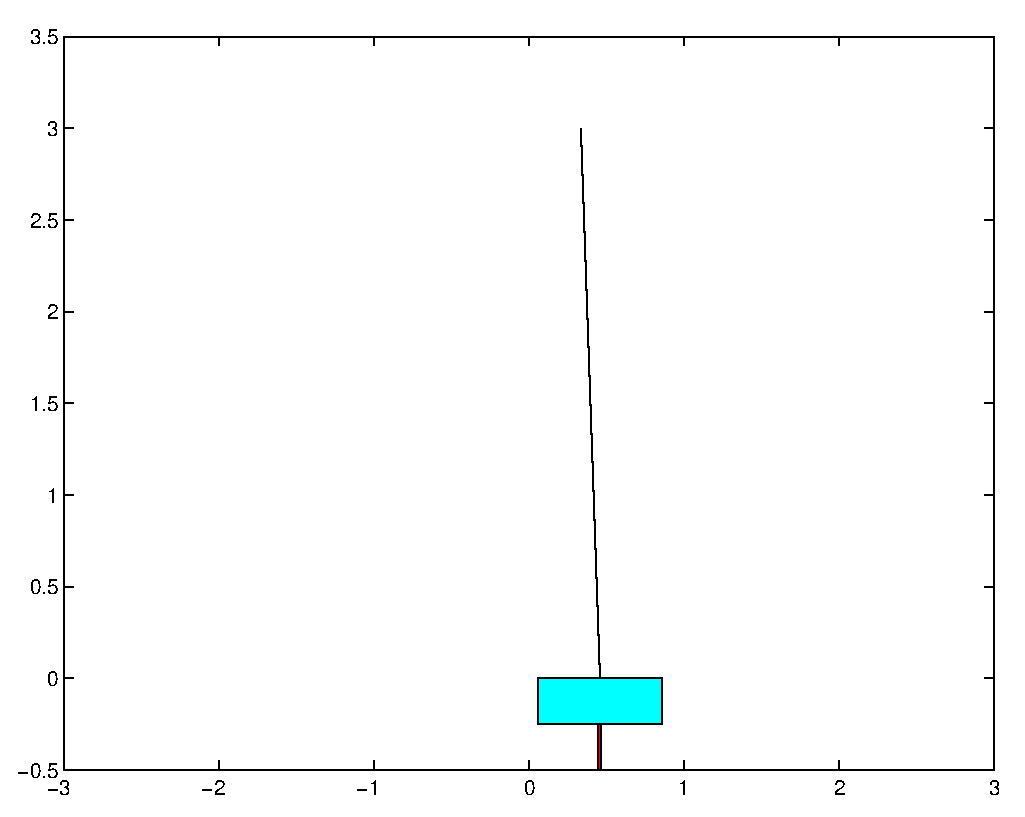
\includegraphics[width=6cm]{cartpole/cart_pole.eps}
\end{center}

We have written a simple simulator for this problem. The simulation 
proceeds in discrete time cycles (steps). \textbf{The state of the cart and pole at any time 
is completely characterized by 4 parameters: the cart position $x$, the 
cart velocity $\dot{x}$, the angle of the pole $\theta$ measured as its deviation 
from the vertical position, and the angular velocity of the pole $\dot{\theta}$.  }
Since it would be simpler to
consider reinforcement learning in a discrete state space,
we have approximated the state space by a discretization that maps 
a state vector $(x,\dot{x}, \theta, \dot{\theta})$ into a number
from 0 to {\tt NUM\_STATES-1}. Your learning algorithm will need to 
deal only with this discretized representation of the states.

\textbf{At every time step, the controller must choose one of two actions -
push (accelerate) the cart right, or push the cart left.}
(To keep the problem simple, there is no {\it do-nothing} action.)
These are represented as actions $0$ and $1$ respectively in the code.  
When the action choice is made, the simulator updates the state parameters 
according to the underlying dynamics, and provides a new discretized state.

\textbf{We will assume that the reward $R(s)$ is a function of the current state only.}
When the pole angle goes beyond a certain limit or when the cart goes
too far out, a negative reward is given, and the system is reinitialized 
randomly. At all other times, the reward is zero.  Your program must learn 
to balance the pole using only the state transitions and rewards observed.
\newpage
\textbf{Task} 

The files for this problem are in {\tt src/cartpole/} directory.
Most of the the code has already been written for you, and you need 
to make changes only to {\tt cartpole.py} in the places specified. This 
file can be run to show a display and to plot a learning curve 
at the end.  There are several details (e.g. convergence criteria) that are also explained inside the code. Use a discount factor of $\gamma = 0.995$.  

 To solve the inverted pendulum problem, you will 
 \begin{itemize}
     \item  Estimate a   model (i.e., transition probabilities and rewards) for the underlying MDP
     \item Solve Bellman's equations for this estimated MDP to obtain a value function
     \item Act greedily with respect to this value function
 \end{itemize}
 
  \textbf{Initially,} the estimated reward of each state is zero,
  and the estimated transition probabilities are uniform (equally likely 
  to end up in any other state).

  \textbf{During the simulation,} you must choose actions at each time step 
  according to some current policy.  As the program goes along taking 
  actions, it will gather observations on transitions and rewards,
  which it can use to get a better estimate of the MDP model.
  
  Since it is inefficient to update the whole estimated MDP after every 
  observation, we will store the state transitions and reward observations 
  each time, and update the model and value function/policy only periodically. 
  Thus, you must maintain counts of the total number of times the 
  transition from state $s_i$ to state $s_j$ using action $a$ has been 
  observed; similarly for the rewards.  Note that the rewards at 
  any state are deterministic, but the state transitions are not because 
  of the discretization of the state space (several different but close
  configurations may map onto the same discretized state).

  \textbf{Each time a failure occurs} (such as if the pole falls over), you should 
  re-estimate the transition probabilities and rewards as the average of 
  the observed values, if any.  Your program should solve Bellman's equation via value iteration 
  to obtain a new value function and optimal policy.  When you do the value iteration, use a 
  convergence criterion to check if the maximum absolute change in the 
  value function on an iteration exceeds some specified tolerance. 

  \textbf{Finally,} consider the entire learning procedure as converged 
  when several consecutive attempts (defined by the parameter 
  {\tt NO\_LEARNING\_THRESHOLD}) to solve Bellman's
  equation all converge in the first iteration. Intuitively, this
  indicates that the estimated model has stopped changing significantly.

  After you implement and execute the reinforcement learning algorithm as specified, include the following items in your write-up:

\begin{itemize}
\item  Plot a learning curve showing the number of time-steps for which the
  pole was balanced on each trial. The starter code already includes plotting codes.
\item  Without changing the random seed, how many trials did it take for the algorithm to converge? (i.e. how many trials does it take before the log number of steps before failure becomes stable?) \\
  Hint: if your solution is correct, the red line on the plot should start to flatten out at about 60 iterations.
\item  Find the line of code that says {\tt np.random.seed}. Set the seed to 1, 2, and 3 and rerun the code for each seed. Describe your observations (you don't need to include the graphs). What do they imply about the algorithm? 

\end{itemize}

\ifnum\solutions=1 {
  \begin{answer}

\end{answer}

} \fi
